\documentclass[a4paper, titlepage]{scrartcl}

\usepackage[ngerman]{babel}
\usepackage[utf8]{inputenc}
\usepackage[T1]{fontenc}
\usepackage{graphicx}
\usepackage{listings}
\usepackage{color}

\definecolor{dkgreen}{rgb}{0,0.6,0}
\definecolor{gray}{rgb}{0.5,0.5,0.5}
\definecolor{mauve}{rgb}{0.58,0,0.82}

\lstset{frame=tb,
  language=Java,
  aboveskip=3mm,
  belowskip=3mm,
  showstringspaces=false,
  columns=flexible,
  basicstyle={\small\ttfamily},
  numbers=none,
  numberstyle=\tiny\color{gray},
  keywordstyle=\color{blue},
  commentstyle=\color{dkgreen},
  stringstyle=\color{mauve},
  breaklines=true,
  breakatwhitespace=true,
  tabsize=3
}


\graphicspath{{./images/}}

\title{UML Dokumentation}
\author{Damien Flury}
\date{27. Februar 2019}

\begin{document}
    \maketitle
    \tableofcontents
    \newpage
    \section{Einführung}
    \section{Klassendiagramme}
    \subsection{Vererbung}
    Bei der Vererbung (engl. Inheritance) von Klassen werden Unterklassen generalisiert. Java
    verfügt im Gegensatz zu zum Beispiel C++ nur über Single Inheritance, das heisst, dass eine Klasse
    jeweils nur von maximal einer anderen Basisklasse erben kann. Dies führt zu einigen Limitierungen,
    vereinfacht den Code jedoch. Somit muss in Java gegebenenfalls auf andere Beziehungen ausgewichen werden,
    wie zum Beispiel die Komposition. Codebeispiel: \ref{InheritanceJava}, grafische Beispiele: Abbildung \ref{VererbungDrawIO}
    und Abbildung \ref{VererbungUmlDesigner}.

    \begin{figure}
        \begin{lstlisting}
    public class Person {
        private final String firstName;
        private final String lastName;
        public Person(String firstName, String lastName) {
            this.firstName = firstName;
            this.lastName = lastName;
        }        
    }

    public final class Employee extends Person {
        private final String teamName;
        public Employee(String firstName, String lastName, string teamName) {
            super(firstName, lastName);
            this.teamName = teamName;
        }
    }
        \end{lstlisting}
    \caption{Vererbung in Java}
    \label{InheritanceJava}
    \end{figure}

    \begin{figure}
        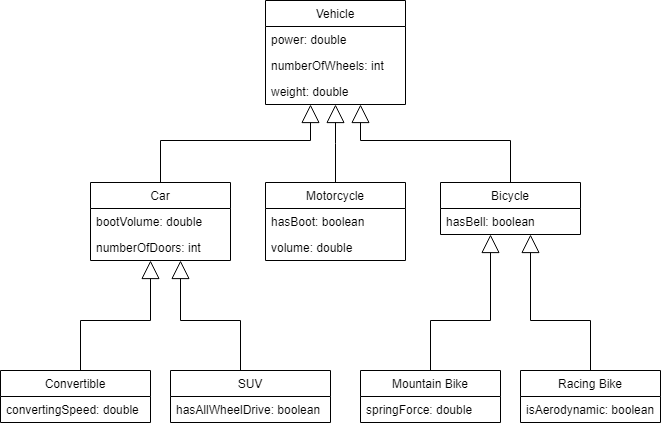
\includegraphics[width=\textwidth]{Klassendiagramm1a}
        \caption{UML-Diagramm mit Vererbung (draw.io)}
        \label{VererbungDrawIO}
    \end{figure}
    \begin{figure}
        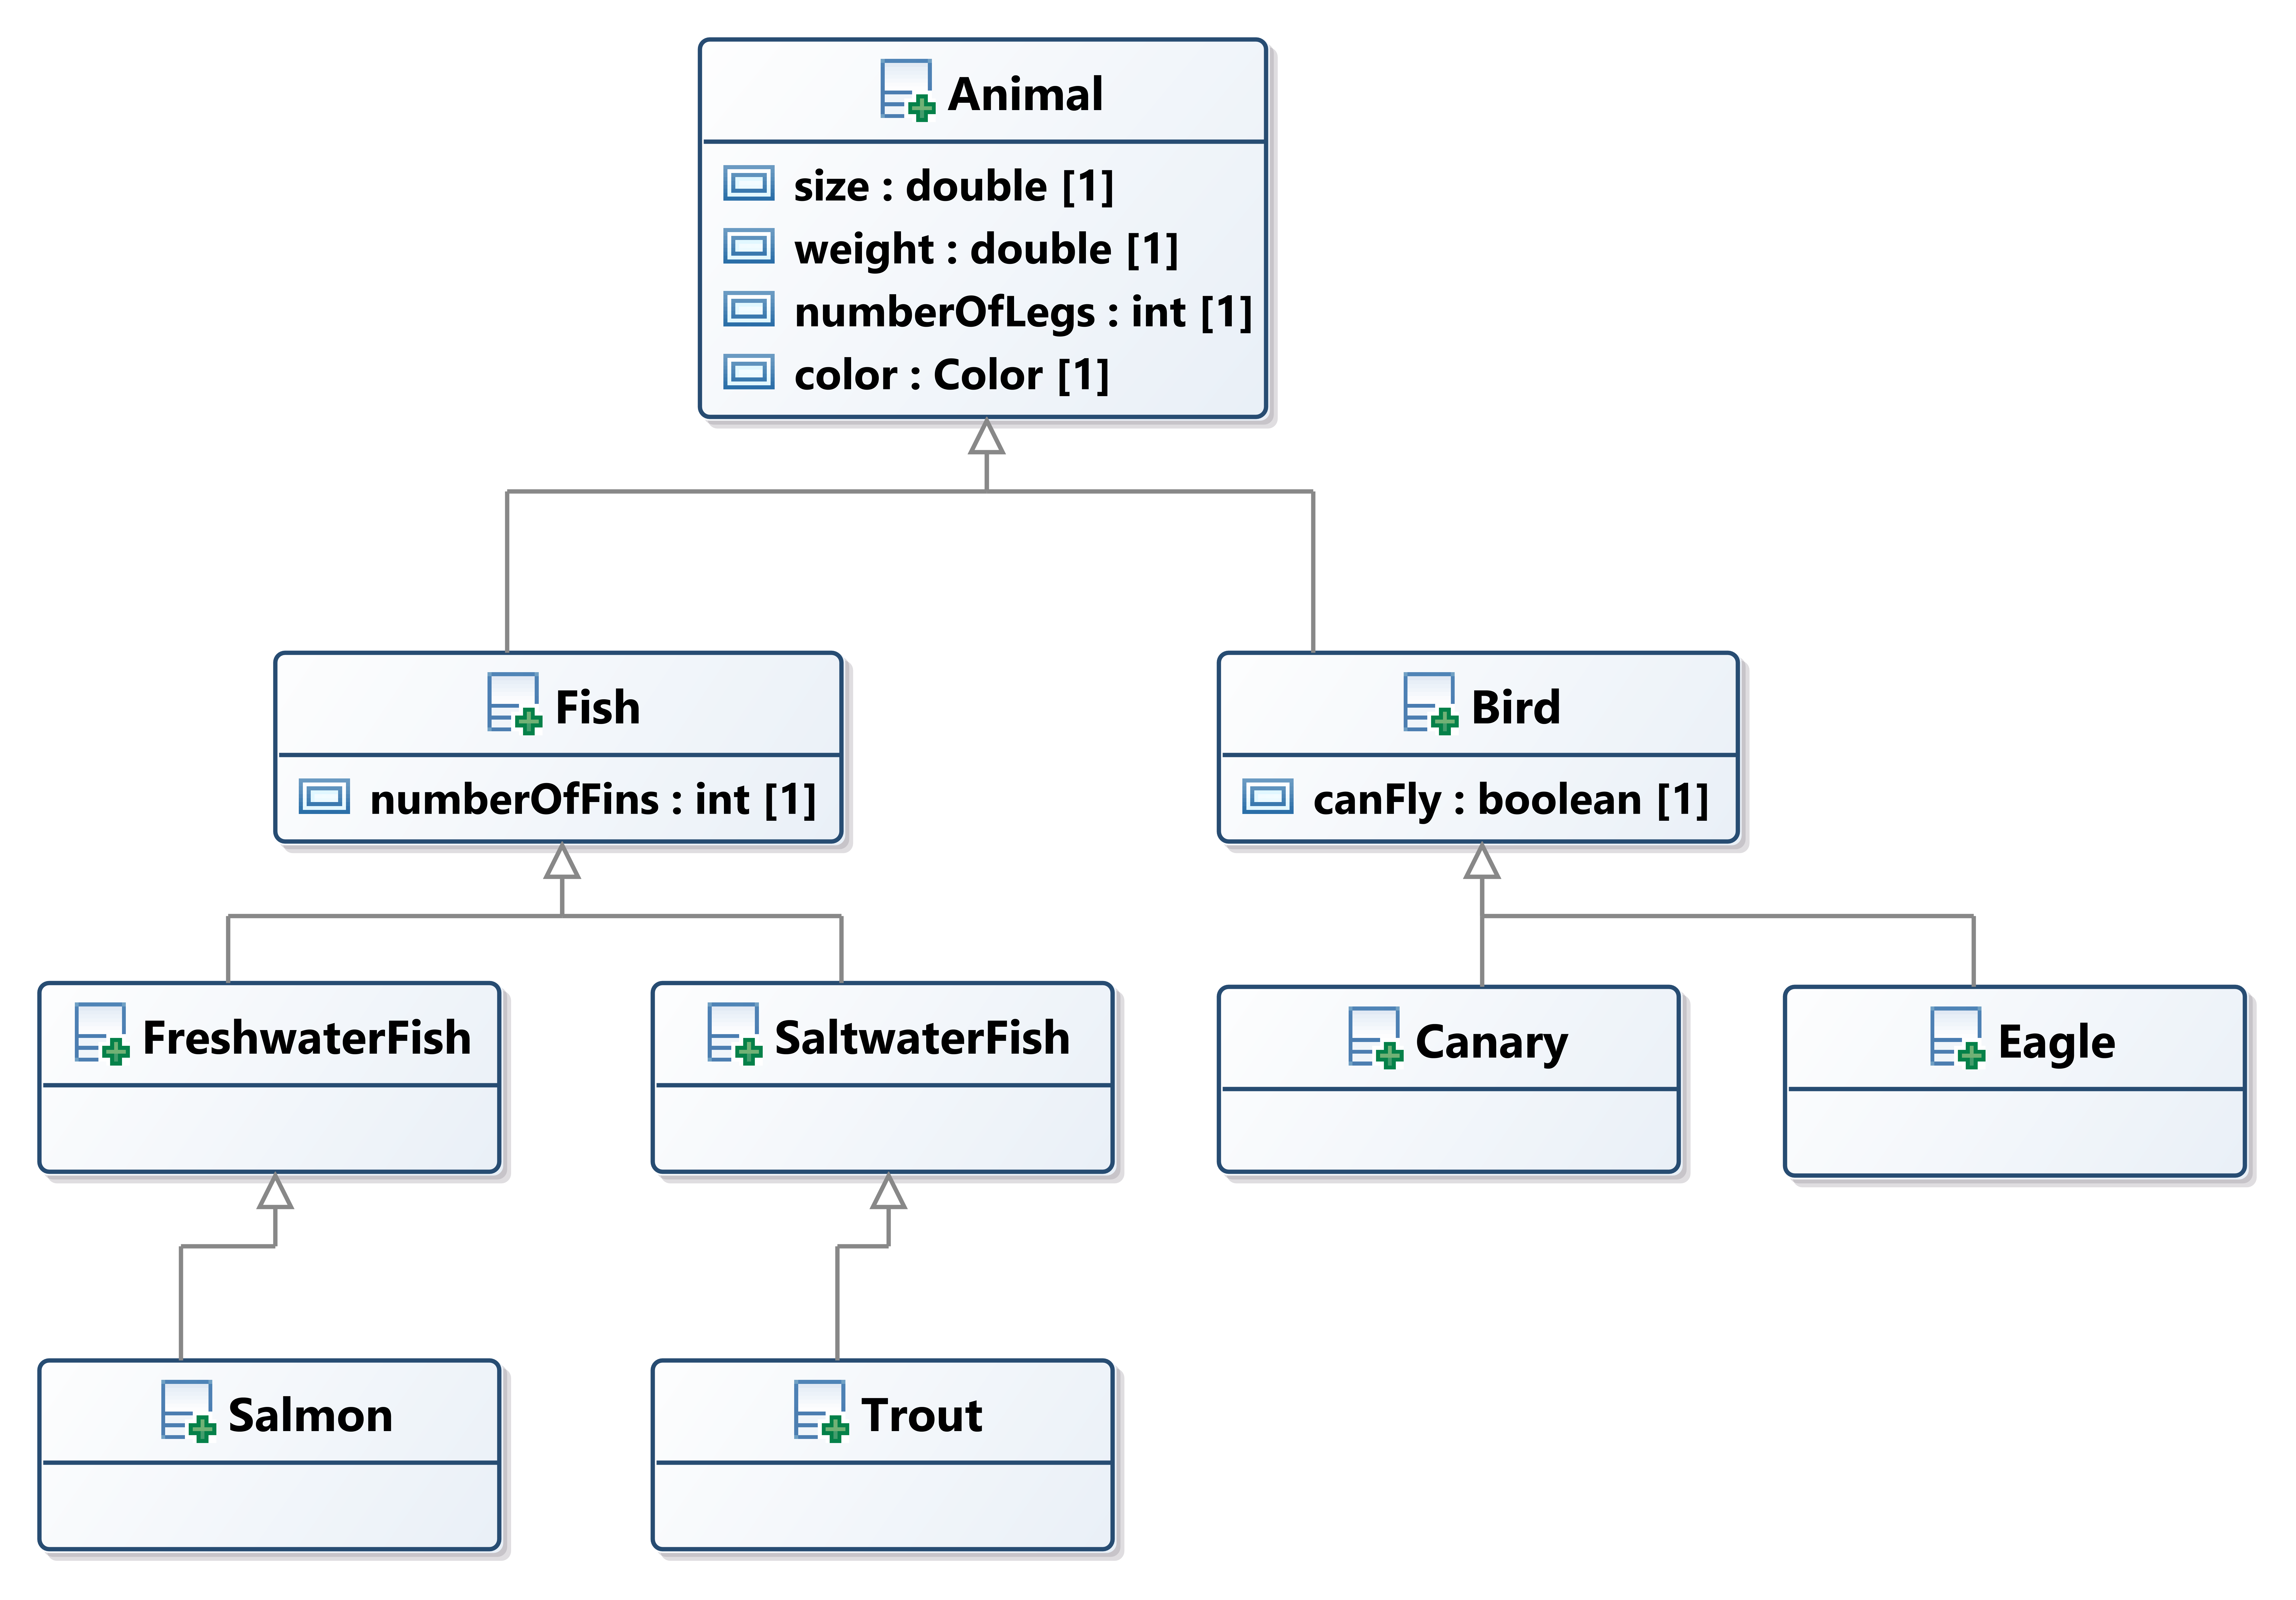
\includegraphics[width=\textwidth]{Klassendiagramm1b}
        \caption{UML-Diagramm mit Vererbung (UML Designer)}
        \label{VererbungUmlDesigner}
    \end{figure}
    
    \subsection{Assoziationen}
    Assoziationen bezeichnen sowohl Besitz- als auch Kennbeziehungen.
    Dies funktioniert im Beispiel von Java häufig anhand des Konstruktors
    oder mithilfe von Setter-Methoden. Codebeispiel: Abbildung \ref{AggregationJava},
    UML-Diagramme sind unter Abbildung \ref{AssoziationenDrawIO} und
    Abbildung \ref{AssoziationenUmlDesigner} zu finden.

    \begin{figure}
    \begin{lstlisting}
    public final class Application {
        public static void main(String[] args) {
            var bike = new Bike();

            // Hier wird dem Driver ein Bike uebergeben:
            var driver = new Driver(bike);
        }
    }

    public final class Driver {
        private final Bike bike;
        public Driver(Bike bike) {
            this.bike = bike
        }        
    }
    \end{lstlisting}
    \caption{Aggregation in Java}
    \label{AggregationJava}
    \end{figure}

    \begin{figure}
        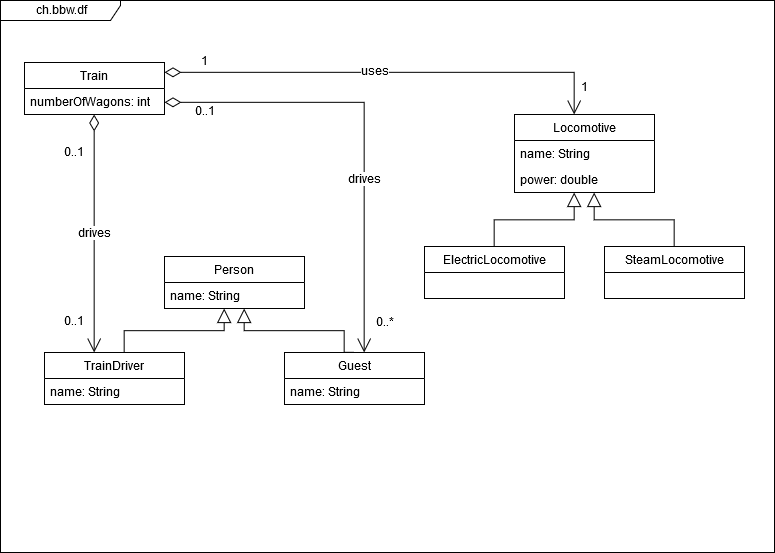
\includegraphics[width=\textwidth]{Assoziationen.png}
        \caption{Klassendiagramm mit Assoziationen (draw.io)}
        \label{AssoziationenDrawIO}
    \end{figure}
    \begin{figure}
        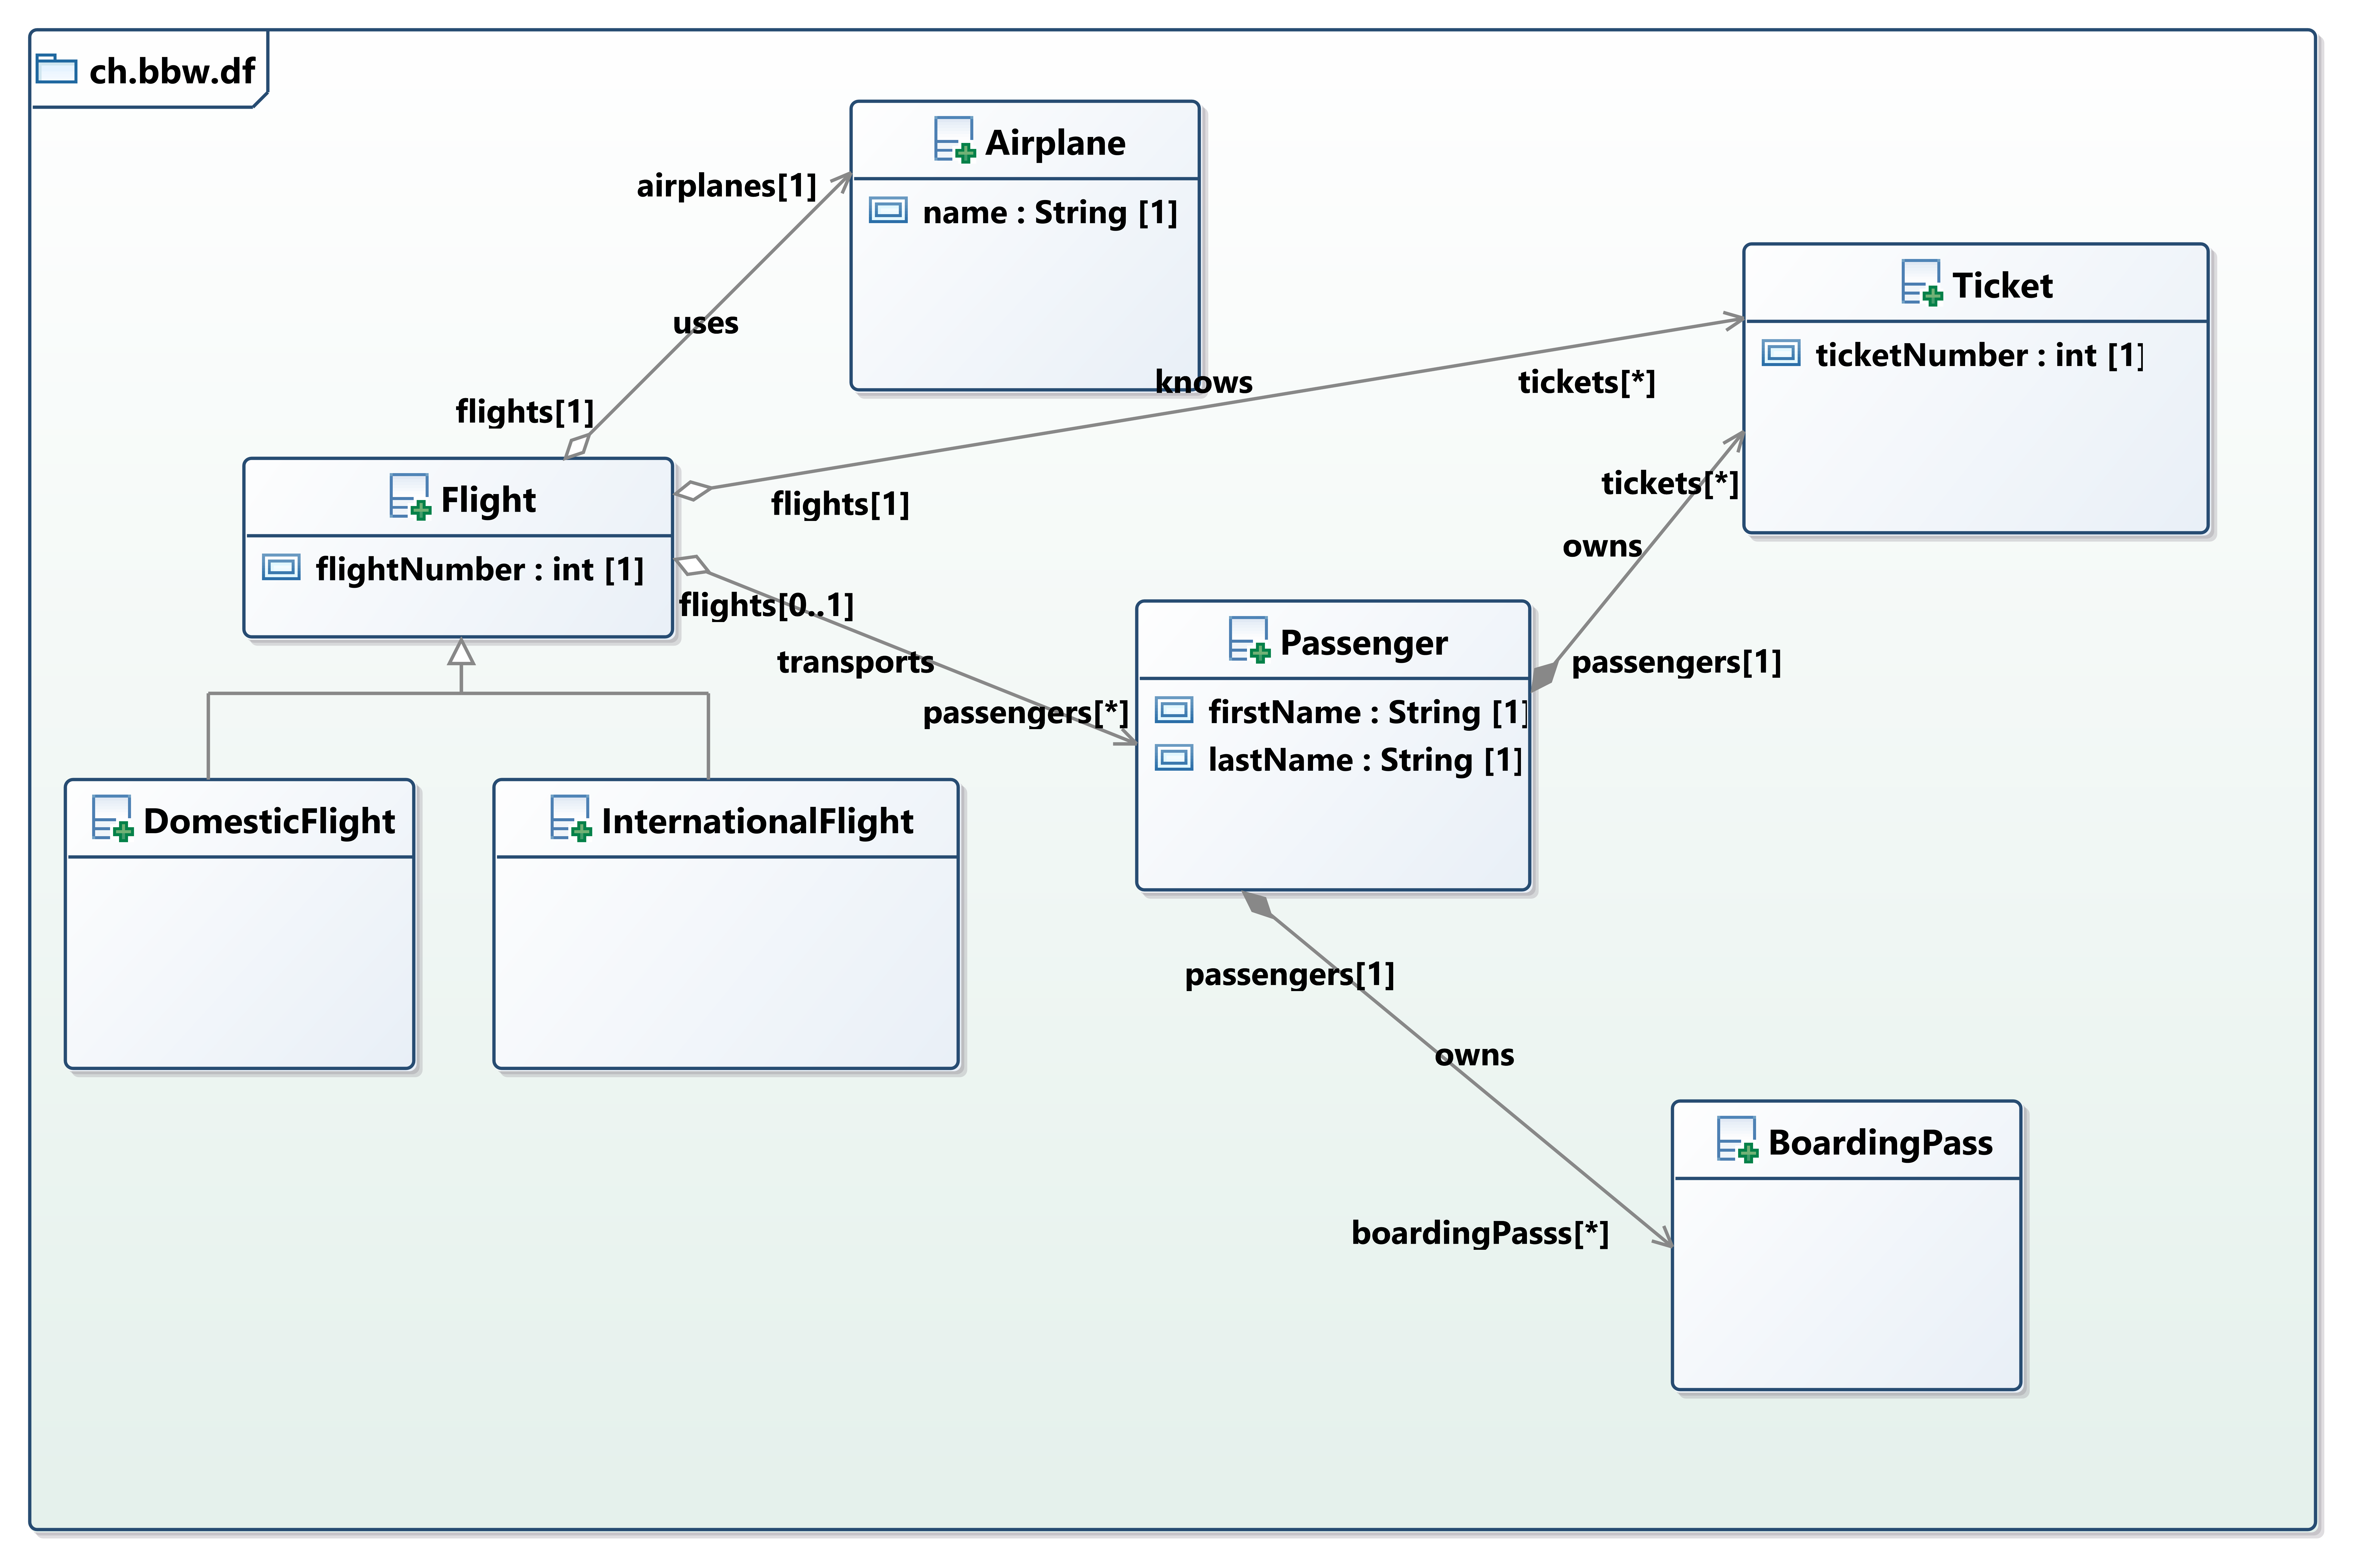
\includegraphics[width=\textwidth]{Assoziationen2.png}
        \caption{Klassendiagramm mit Assoziationen (UML Designer)}
        \label{AssoziationenUmlDesigner}
    \end{figure}

    \section{Use Case Diagram}
    Das Use Case Diagram bietet die Möglichkeit, Benutzerinteraktion mit
    der Applikation zu repräsentieren. Zum ersten Mal vorgestellt wurde
    es an einer Konferenz in 1987 von Jacobson und findet heutzutage häufig
    einen Platz in unterschiedlichen Softwareteams mit diversen Programmiersprachen.
    Beispiele: Abbildung \ref{UseCaseDrawIO} und Abbildung \ref{UseCaseVisio}
    \begin{figure}
        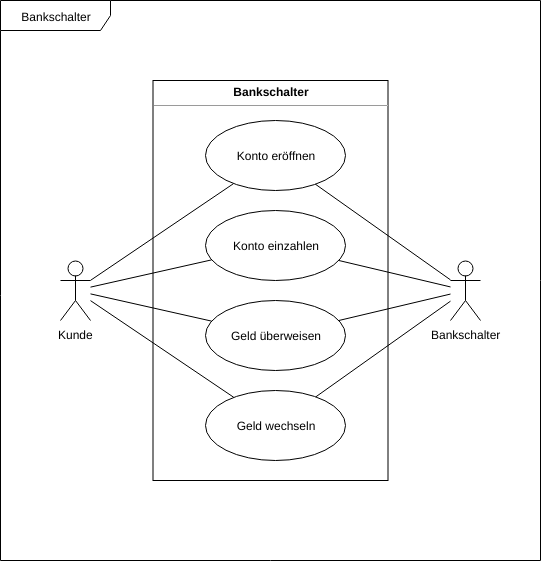
\includegraphics[width=\textwidth]{Anwendungsfalldiagramm1a.png}
        \caption{Use Case Diagram (draw.io)}
        \label{UseCaseDrawIO}
    \end{figure}
    \begin{figure}
        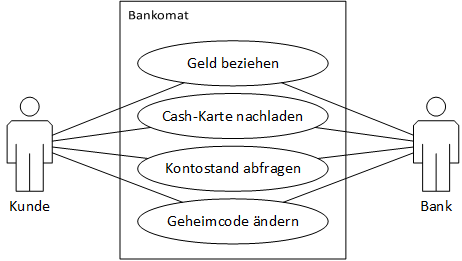
\includegraphics[width=\textwidth]{Anwendungsfalldiagramm1c.png}
        \caption{Use Case Diagram (Microsoft Visio)}
        \label{UseCaseVisio}
    \end{figure}

    \section{Aktivitätsdiagramm}
    Mithilfe des Aktivitätsdiagramms kann man Abläufe, Aktionen und
    Kontrollflüsse beschreiben.

    Häufig werden durch Aktivitätsdiagramme einzelne Use Cases genauer
    beschrieben. Das Aktivitätsdiagramm ermöglicht hier die Darstellung
    von ein wenig komplexeren Abläufen mit Falls-Verzweigungen, Wiederholungen
    und anderen Ausnahmen.
    Beispiele: Abbildung \ref{AktivitaetsdiagrammDrawIO} und Abbildung \ref{AktivitaetsdiagrammUmlet}
    \begin{figure}
        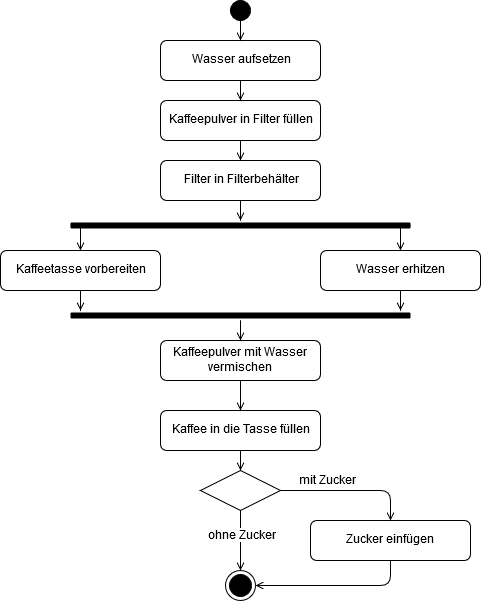
\includegraphics[width=\textwidth]{Aktivitaetsdiagramm1a.png}
        \caption{Aktivitätsdiagramm (draw.io)}
        \label{AktivitaetsdiagrammDrawIO}
    \end{figure}
    \begin{figure}
        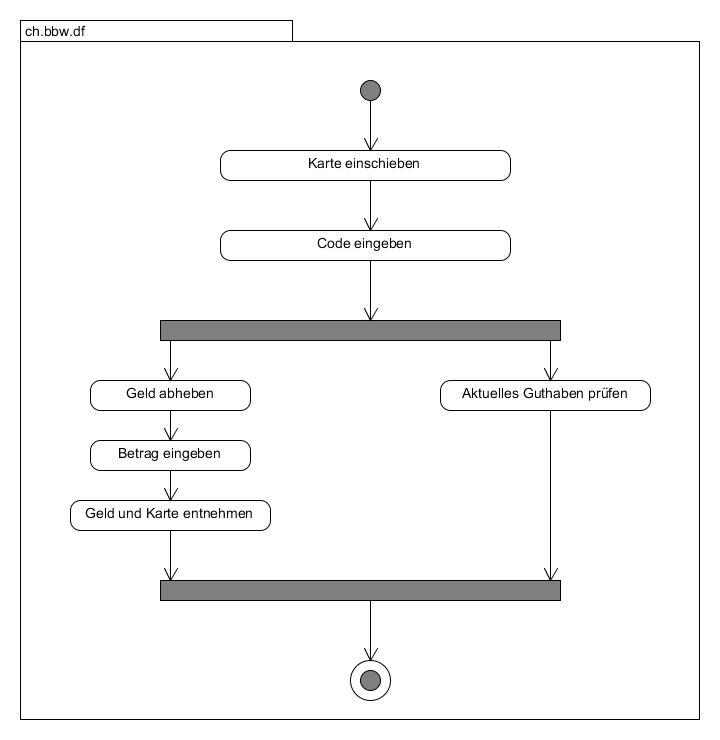
\includegraphics[width=\textwidth]{Aktivitaetsdiagramm1b.png}
        \caption{Aktivitätsdiagramm (UMLet)}
        \label{AktivitaetsdiagrammUmlet}
    \end{figure}

    \section{Fazit zu den Tools}
    \subsection{Draw.io}
    Draw.io ermöglicht das Zeichnen von vielen verschiedenen Diagrammen und
    hat meine Bedürfnisse für alle Aufgabenstellung erfüllt. Die Benutzeroberfläche
    bietet viele Möglichkeiten und wird nach einer Zeit ziemlich intuitiv und einfach.
    
    Ausserdem ist Draw.io eine Webapplikation, benötigt also keinen Download und
    hat direkte Unterstützung von Google Drive. 
    
    Draw.io ist mit Abstand mein Lieblingstool, da es viele Möglichkeiten benutzerfreundlich
    bereitstellt.
    
    \subsection{Visio 2013}
    Visio bietet viele Möglichkeiten, ist jedoch meiner Meinung nach nicht
    sehr benutzerfreundlich. Ausserdem benötigt die Software eine teure Lizenz
    und läuft nur auf Microsoft Windows. Das Endprodukt finde ich persönlich
    eher unbefriedigend und qualitativ nicht so hochwertig wie das von anderen Tools.

    \subsection{UML Designer}
    UML Designer bietet eine hohe Variation von Möglichkeiten, ist jedoch besonders
    am Anfang sehr kompliziert. Ausserdem ist alles sehr Java- und Eclipsebasiert,
    somit denke ich, dass UML Designer für andere Sprachen und Entwicklungsumgebungen
    nicht die beste Lösung ist.

    Das Endprodukt finde ich besonders ansprechend und gewinnt deshalb unter allen Tools.

    \subsection{UMLet}
    UMLet bietet sehr wenige Möglichkeiten von Anfang an. Während Klassendiagramme
    relativ einfach umzusetzen sind, sind Aktivitätsdiagramme sehr aufwendig (aber
    nicht unmöglich). Ich war mir dies leider im Voraus nicht bewusst und habe somit
    ein Aktivitätsdiagramm mithilfe von UMLet erstellt. Das integrierte Scripting-Tool
    ist sehr mächtig und erlaubt die Erzeugung von komplexeren Formen, ist jedoch
    kompliziert und man findet wenig Dokumentation im Internet. 
    
\end{document}